\documentclass[border=3pt]{standalone}
\usepackage[T1]{fontenc}
\usepackage{lmodern}
\usepackage{amsmath,amssymb}
\usepackage{tikz}
\usepackage{pgfplots}
\pgfplotsset{compat=1.17}
\usepgfplotslibrary{groupplots}
\usetikzlibrary{arrows.meta,calc,positioning,fit,backgrounds}

% UAV-based tracking: scale variation and camera motion, and what they require from detection and tracking.
\newcommand{\car}[3]{% position, length, color
  \fill[#3, rounded corners=0.4pt] ($#1-(#2/2,#2/4)$) rectangle ($#1+(#2/2,#2/4)$);}
\newcommand{\dbox}[3][]{% detection box around a car: [style] position, length
  \draw[orange!85!black, line width=0.6pt, #1] ($#2-(#3/2+0.05,#3/4+0.05)$) rectangle ($#2+(#3/2+0.05,#3/4+0.05)$);}
\begin{document}
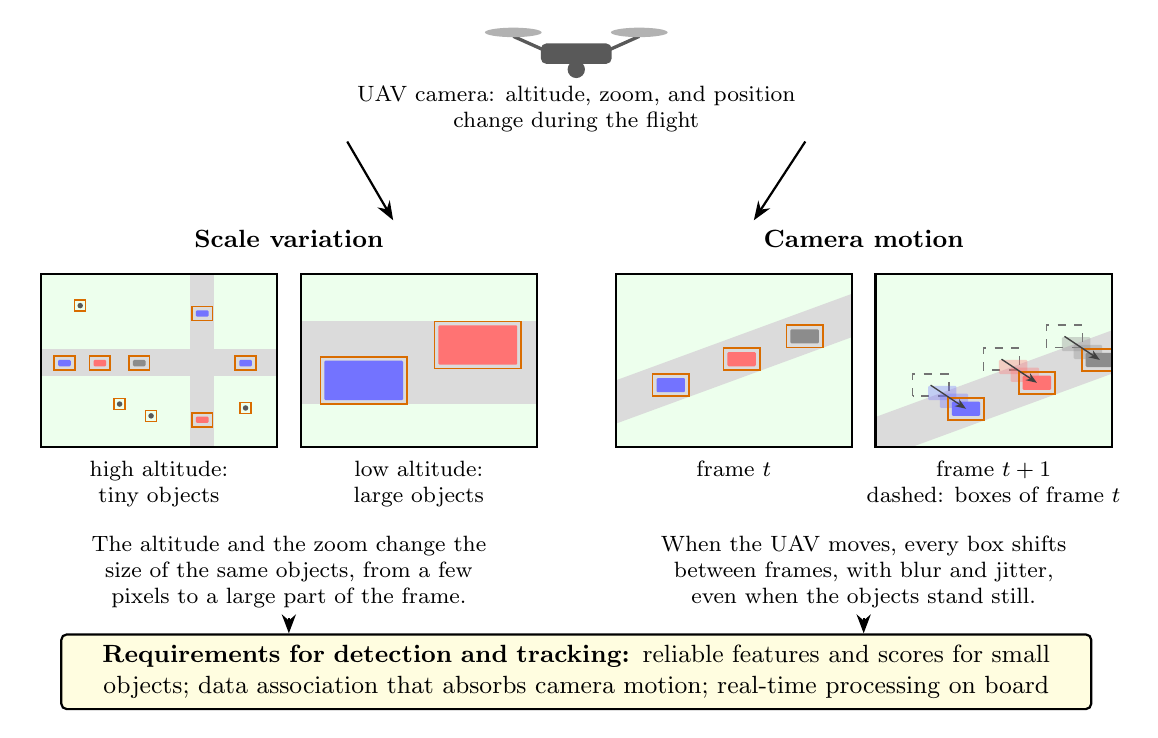
\begin{tikzpicture}[
  font=\small,
  frame/.style={fill=green!7},
  border/.style={draw, thick},
  road/.style={fill=gray!28},
  hdr/.style={font=\small\bfseries, align=center},
  note/.style={font=\footnotesize, align=center, text width=64mm, execute at begin node={\hyphenpenalty10000\relax}},
  flab/.style={font=\footnotesize, align=center, below=0.5mm},
  res/.style={draw, thick, rounded corners=2pt, fill=yellow!12, align=center, text width=128mm, inner sep=4pt},
  arr/.style={-{Stealth[length=2.4mm]}, thick}]
% ---------- UAV ----------
\begin{scope}[shift={(6.8,1.0)}]
  \draw[black!65, line width=1.2pt] (-0.42,0.05) -- (-0.8,0.22) (0.42,0.05) -- (0.8,0.22);
  \fill[black!30] (-0.8,0.27) ellipse (0.36 and 0.06);
  \fill[black!30] (0.8,0.27) ellipse (0.36 and 0.06);
  \fill[black!65, rounded corners=2pt] (-0.45,-0.13) rectangle (0.45,0.13);
  \fill[black!65] (0,-0.2) circle (0.11);
\end{scope}
% ---------- headers ----------
\node[hdr] (hs) at (3.15,-1.35) {Scale variation};
\node[hdr] (hm) at (10.45,-1.35) {Camera motion};
\node[font=\footnotesize, align=center] (ul) at (6.8,0.3) {UAV camera: altitude, zoom, and position\\ change during the flight};
\draw[arr] (ul.south west) -- (hs.north east);
\draw[arr] (ul.south east) -- (hm.north west);
% ---------- scale variation: high altitude ----------
\begin{scope}[shift={(0,-4.0)}]
  \draw[frame] (0,0) rectangle (3,2.2);
  \begin{scope}
    \clip (0,0) rectangle (3,2.2);
    \fill[road] (0,0.9) rectangle (3,1.25); \fill[road] (1.9,0) rectangle (2.2,2.2);
    \foreach \x/\c in {0.3/blue!55, 0.75/red!55, 1.25/black!45, 2.6/blue!55} {
      \car{(\x,1.07)}{0.16}{\c} \dbox{(\x,1.07)}{0.16}}
    \foreach \y/\c in {0.35/red!55, 1.7/blue!55} {\car{(2.05,\y)}{0.16}{\c} \dbox{(2.05,\y)}{0.16}}
    \foreach \px/\py in {0.5/1.8, 1.4/0.4, 2.6/0.5, 1.0/0.55} {
      \fill[black!65] (\px,\py) circle (0.035);
      \draw[orange!85!black, line width=0.5pt] (\px-0.07,\py-0.07) rectangle (\px+0.07,\py+0.07);}
  \end{scope}
  \draw[border] (0,0) rectangle (3,2.2);
  \node[flab] at (1.5,0) {high altitude:\\ tiny objects};
\end{scope}
% ---------- scale variation: low altitude ----------
\begin{scope}[shift={(3.3,-4.0)}]
  \draw[frame] (0,0) rectangle (3,2.2);
  \begin{scope}
    \clip (0,0) rectangle (3,2.2);
    \fill[road] (0,0.55) rectangle (3,1.6);
    \car{(0.8,0.85)}{1.0}{blue!55} \dbox{(0.8,0.85)}{1.0}
    \car{(2.25,1.3)}{1.0}{red!55} \dbox{(2.25,1.3)}{1.0}
  \end{scope}
  \draw[border] (0,0) rectangle (3,2.2);
  \node[flab] at (1.5,0) {low altitude:\\ large objects};
\end{scope}
% ---------- camera motion: frame t ----------
\begin{scope}[shift={(7.3,-4.0)}]
  \draw[frame] (0,0) rectangle (3,2.2);
  \begin{scope}
    \clip (0,0) rectangle (3,2.2);
    \fill[road] (0,0.3) -- (0,0.85) -- (3,1.95) -- (3,1.4) -- cycle;
    \foreach \px/\py/\c in {0.7/0.79/blue!55, 1.6/1.12/red!55, 2.4/1.41/black!45} {\car{(\px,\py)}{0.36}{\c} \dbox{(\px,\py)}{0.36}}
  \end{scope}
  \draw[border] (0,0) rectangle (3,2.2);
  \node[flab] at (1.5,0) {frame $t$\\ \strut};
\end{scope}
% ---------- camera motion: frame t+1 (scene shifted, blurred) ----------
\begin{scope}[shift={(10.6,-4.0)}]
  \draw[frame] (0,0) rectangle (3,2.2);
  \begin{scope}
    \clip (0,0) rectangle (3,2.2);
    \fill[road] (-0.2,-0.238) -- (-0.2,0.312) -- (3.2,1.558) -- (3.2,1.008) -- cycle;
    \foreach \px/\py/\c in {0.7/0.79/blue!55, 1.6/1.12/red!55, 2.4/1.41/black!45} {
      \coordinate (P) at (\px,\py); \coordinate (Q) at (\px+0.45,\py-0.3);
      \dbox[dashed, black!55]{(P)}{0.36}
      \foreach \f in {0.33,0.66} {\coordinate (G) at ($(P)!\f!(Q)$); \begin{scope}[opacity=0.35]\car{(G)}{0.36}{\c}\end{scope}}
      \car{(Q)}{0.36}{\c} \dbox{(Q)}{0.36}
      \draw[-{Stealth[length=1.4mm]}, black!75, line width=0.5pt] (P) -- (Q);}
  \end{scope}
  \draw[border] (0,0) rectangle (3,2.2);
  \node[flab] at (1.5,0) {frame $t+1$\\ dashed: boxes of frame $t$};
\end{scope}
% ---------- explanations ----------
\node[note, anchor=north] (ns) at (3.15,-5.0) {The altitude and the zoom change the size of the same objects, from a few
  pixels to a large part of the frame.};
\node[note, anchor=north] (nm) at (10.45,-5.0) {When the UAV moves, every box shifts between frames, with blur and jitter,
  even when the objects stand still.};
\node[res] (req) at (6.8,-6.85) {\textbf{Requirements for detection and tracking:} reliable features and scores
  for small objects; data association that absorbs camera motion; real-time processing on board};
\draw[arr] (ns.south) -- (ns.south |- req.north);
\draw[arr] (nm.south) -- (nm.south |- req.north);
\end{tikzpicture}
\end{document}
